\documentclass[12pt, a4paper, UTF8, oneside]{ctexart}

\newcommand{\chuhao}{42pt}
\newcommand{\xiaochu}{36pt}

\newcommand{\yihao}{26pt}
\newcommand{\xiaoyi}{24pt}

\newcommand{\erhao}{22pt}
\newcommand{\xiaoer}{18pt}

\newcommand{\sanhao}{16pt}
\newcommand{\xiaosan}{15pt}

\newcommand{\sihao}{14pt}
\newcommand{\xiaosi}{12pt}

\newcommand{\wuhao}{10.5pt}
\newcommand{\xiaowu}{9pt}

\newcommand{\liuhao}{7.5pt}
\newcommand{\xiaoliu}{6.5pt}

\newcommand{\qihao}{5.5pt}

\newcommand{\bahao}{5pt}

\setmainfont{Times New Roman}

\usepackage{geometry}
\geometry{left=3cm, right=2cm, top=3cm, bottom=2.5cm}

\usepackage{graphicx}
\graphicspath{{pics/}}

\usepackage{fancyhdr}
\pagestyle{fancy}
\fancyhf{} 
\fancyhead[C]{
\includegraphics[scale=0.5]{logo.png}}
\fancyfoot[C]{\thepage}
\renewcommand{\headrulewidth}{0.1mm} 
\renewcommand{\footrulewidth}{0.1mm}

\usepackage{datetime}
\usepackage[cmyk]{xcolor}
\usepackage{array}
\usepackage{verbatim}
\usepackage{placeins}

\usepackage{listings}
\lstset{
    basicstyle          =   \linespread{1.2}\selectfont\ttfamily,
    keywordstyle        =   \color{blue},
    commentstyle        =   \color{gray},
    stringstyle         =   \color{green!50!black},
    columns             =   flexible,
    numbers             =   left,
    numberstyle         =   \footnotesize,
    showspaces          =   false,
    showstringspaces    =   false,
    captionpos          =   t,
    frame               =   lrtb,
    breaklines          =   true,
    basewidth           =   0.5em,
    backgroundcolor     =   \color[RGB]{245,245,244},
}

\lstdefinestyle{Matlab}{
    language = Matlab,
}

\begin{document}
    \newcommand{\course}{
    数字信号处理
}
\newcommand{\college}{
    自动化科学与电气工程学院
}
\newcommand{\major}{
    自动化
}
\newcommand{\StudentID}{
    XXXXXXXX
}
\newcommand{\name}{
    XX
}
\newcommand{\teacher}{
    XX
}

\newcommand{\extimes}{
    X
}
\newcommand{\exname}{
    XXXX
}
\newcommand{\extime}{
    X月XX日
}
\newcommand{\classmate}{
    无
}
    \renewcommand{\maketitle}{
    \begin{titlepage}

        \begin{minipage}[c]{0.5\linewidth}
            
\includegraphics[scale=1.0]{BUAAr.png}
        \end{minipage}
        \hfill
        \begin{minipage}[c]{0.3\linewidth}
            \heiti \fontsize{\sihao}{1em} \selectfont 成 \quad 绩 \quad \underline{\qquad\qquad}
        \end{minipage}
        
        \begin{center}
            \vspace{0.5cm}
            
\includegraphics[scale=0.4]{BUAA.png} \\
            \vspace{2cm}
            \heiti \fontsize{\xiaochu}{1em} \selectfont \course \\
            \vspace{0.5cm}
            \songti \fontsize{32pt}{1em} \selectfont \bf 实验报告
        \end{center}
        \vspace{3.5cm}
        
        \begin{center}
            \heiti \fontsize{\xiaosan}{1em} \selectfont
            \makebox[10em][s]{院(系)名称} \quad \underline{\makebox[16em][c]{\college}}\\[1em]
            \makebox[10em][s]{专业名称} \quad \underline{\makebox[16em][c]{\major}}\\[1em]
            \makebox[10em][s]{学生学号} \quad \underline{\makebox[16em][c]{\StudentID}}\\[1em]
            \makebox[10em][s]{学生姓名} \quad \underline{\makebox[16em][c]{\name}}\\[1em]
            \makebox[10em][s]{指导教师} \quad \underline{\makebox[16em][c]{\teacher}}
        \end{center}

        \begin{table}[b]
            \begin{center}
                \heiti \fontsize{\xiaosan}{1em} \selectfont \number\year 年 \number\month 月
            \end{center}
        \end{table}
    \end{titlepage}
}
    \maketitle

    \linespread{1.5} \selectfont

    \begin{center}
        \heiti \fontsize{\sanhao}{1em} 实验\extimes \qquad \exname
        \vspace{0.3cm}
    \end{center}

    {
    \heiti \fontsize{\sihao}{1em}
    \begin{minipage}[b]{0.4\linewidth}
        \begin{center}
            实验时间\underline{\makebox[6em][c]{\extime}}
        \end{center}
    \end{minipage}
    \hfill
    \begin{minipage}[b]{0.4\linewidth}
        \begin{center}
            同组同学\underline{\makebox[6em][c]{\classmate}}
        \end{center}
    \end{minipage}
    }
    \vspace{0.5cm}
    
    \begin{flushleft}
        \heiti\fontsize{\sihao}{1em}一、实验目的
    \end{flushleft}

    \begin{enumerate}
    \item 熟悉 MATLAB 编程环境、掌握 MATLAB 编程特点、
            了解数字信号处理工具箱;掌握常用图形绘制与标注方法。
    \item 掌握基于计算机软件的正弦序列、指数序列、
            复正弦序列、多频正弦序列、含噪声序列的生成方法。
    \item 掌握 MATLAB 的函数编程方法,掌握滑动平均滤波原理及实现方法,
    掌握窗口长度对滑动平均结果的影响规律。
\end{enumerate}
    
    \begin{flushleft}
        \heiti\fontsize{\sihao}{1em}二、实验过程与结果
    \end{flushleft}

    \begin{enumerate}
    \item MATLAB 编程生成正弦序列
\end{enumerate}
\lstinputlisting[
    style = Matlab,
    caption = {正弦序列}
]{code/sin_list.m}
\begin{figure}[ht]
    \centering
    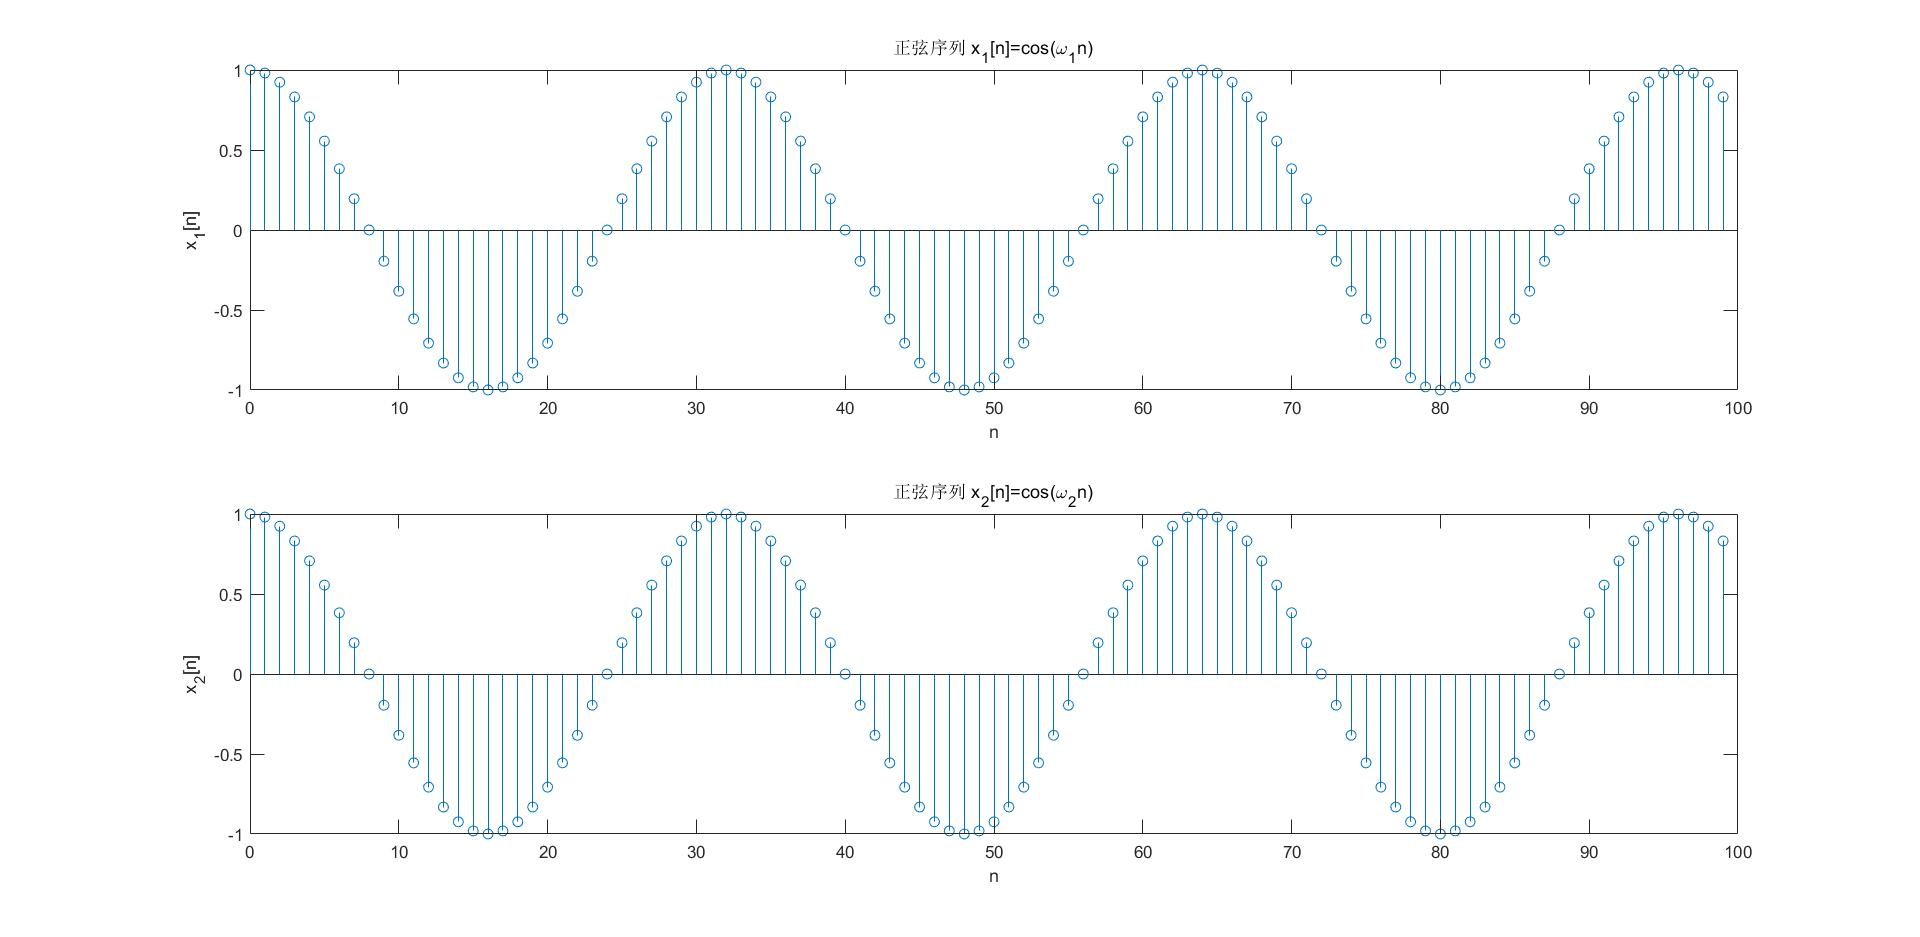
\includegraphics[width=1\linewidth]{sin.jpg}
    \caption{正弦序列}
\end{figure}

    \begin{flushleft}
        \heiti\fontsize{\sihao}{1em}三、结果分析与实验结论
    \end{flushleft}
    
    \textbf{留数定理}

函数\(f(z)\)在区域\(D\)内除有限个孤立奇点\(\{z_n\}\)外解析, \(C\)是\(D\)内包含这些奇点的简单闭曲线, 则

\begin{equation}
    \frac1{2\pi i}\int_Cf(z)\,\text{d} z=\sum\limits_{k=1}^n\text{Res}(f(z),z_k)
\end{equation}

\textbf{可控标准形}

\begin{equation}
    \dot x=
    \begin{bmatrix}
        0& 1  \\
        && 1 \\
        &&&\ddots \\
        &&&&1\\
        -a_0 & -a_1 & -a_2 & \cdots & -a_{n-1}
    \end{bmatrix}
    x+
    \begin{bmatrix}
        0\\
        0\\
        \vdots\\
        0\\
        1
    \end{bmatrix}u
\end{equation}
    
    \begin{flushleft}
        \heiti\fontsize{\sihao}{1em}四、收获、体会及建议
    \end{flushleft}

    \input{content/4.tex}
    
\end{document}